%!TEX root = ../template.tex
%%%%%%%%%%%%%%%%%%%%%%%%%%%%%%%%%%%%%%%%%%%%%%%%%%%%%%%%%%%%%%%%%%%
%% chapter1.tex
%% NOVA thesis document file
%%
%% Chapter with introduciton
%%%%%%%%%%%%%%%%%%%%%%%%%%%%%%%%%%%%%%%%%%%%%%%%%%%%%%%%%%%%%%%%%%%


\chapter{Conclusions and Future Work}
\label{cha:conclusions_and_future_work}

\section{Results Analysis}
\label{sec:results_analysis}

\begin{figure}[htbp]
	\centering
	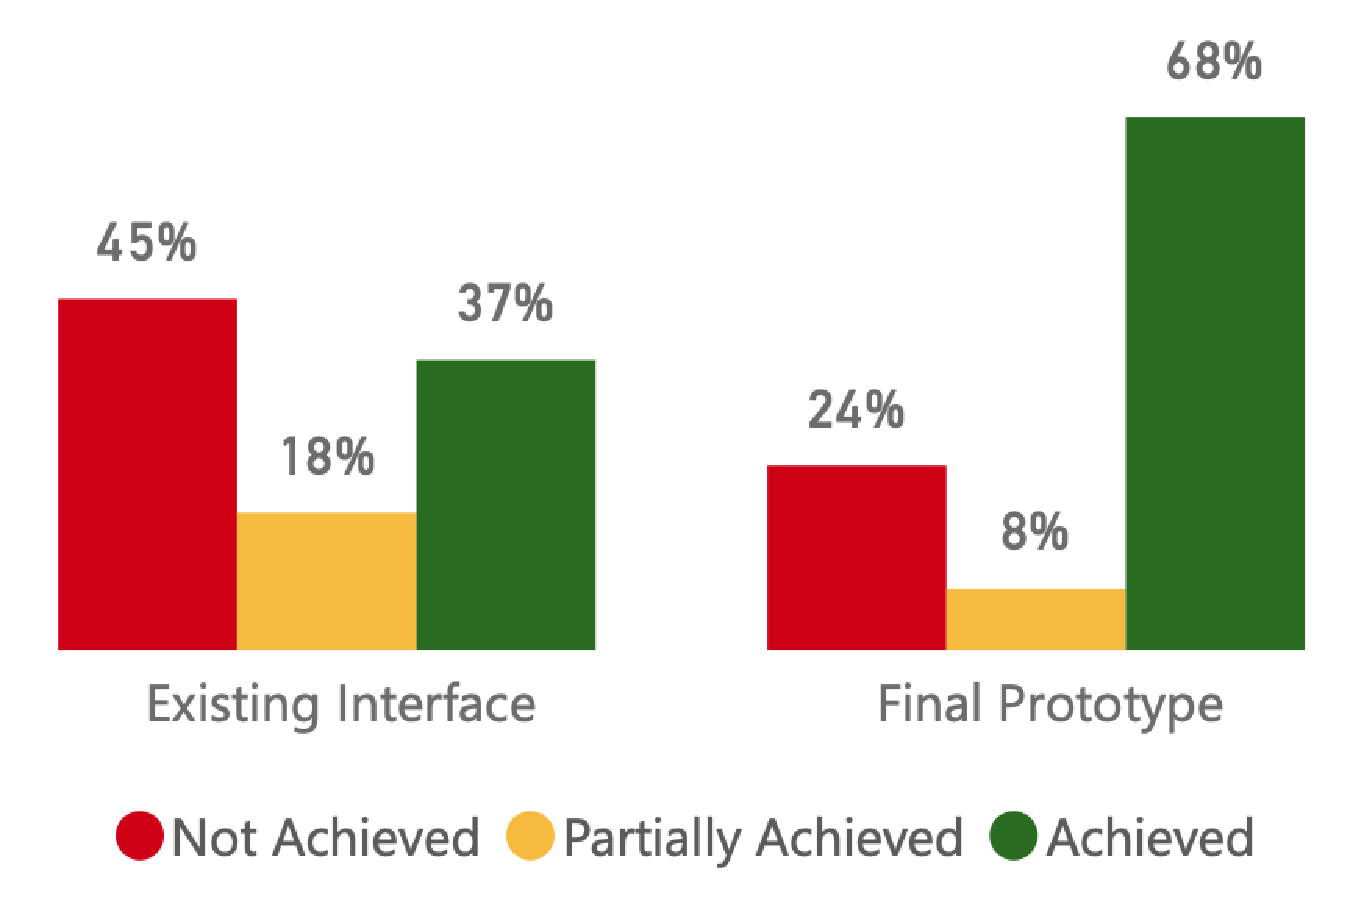
\includegraphics[height=2.2in]{total-effectiveness-comparison}
	\caption{Effectiveness Comparison between the existing interface and the final prototype.}
	\label{fig:totalEffectivenessComparison}
\end{figure}

\begin{figure}[htbp]
	\centering
	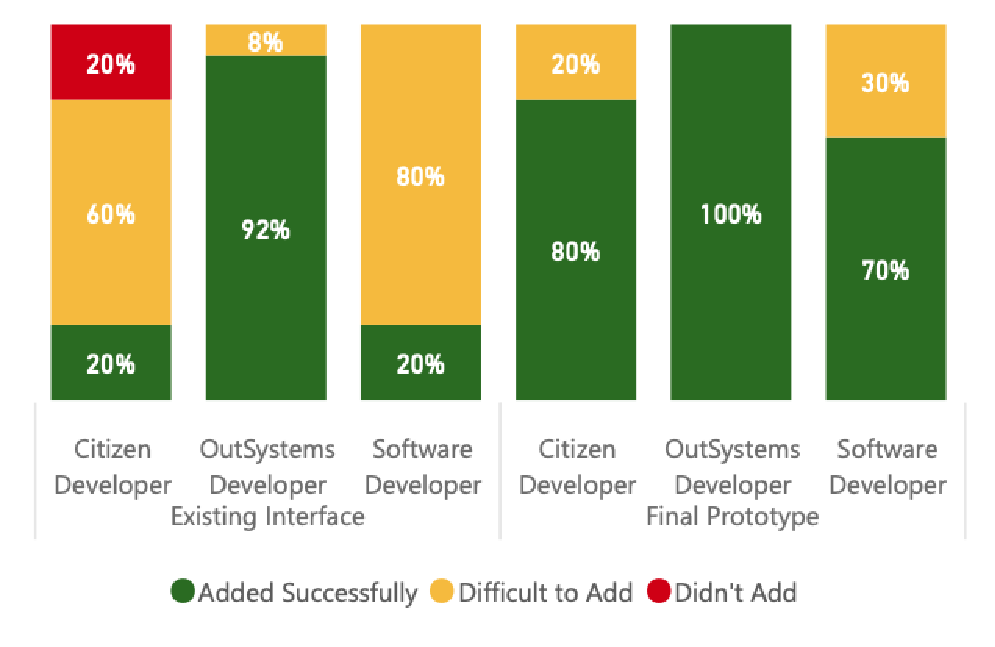
\includegraphics[height=2.0in]{add-calculated-attribute-comparison}
	\caption{Effectiveness Comparison between the existing interface and the final prototype.}
	\label{fig:addCalculatedAttributeComparison}
\end{figure}

\begin{figure}[tb]
    \centering
    \subcaptionbox{Add calculated attribute\label{fig:addCalculatedAttributeComparison}}%
      {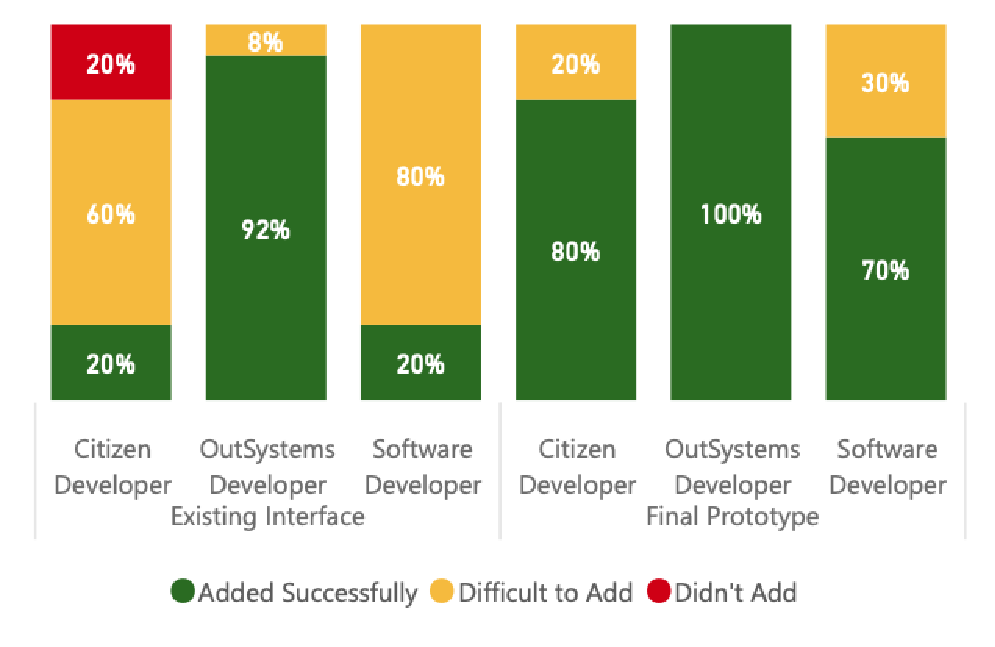
\includegraphics[width=0.5\linewidth]{add-calculated-attribute-comparison}}%
    \subcaptionbox{Foreign key selection\label{fig:foreignKeySelectionComparison}}%
    {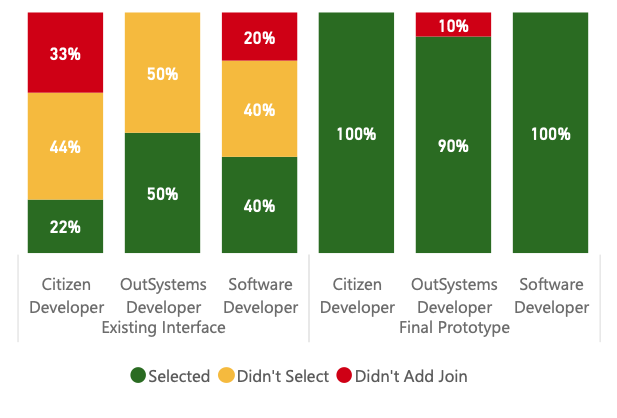
\includegraphics[width=0.5\linewidth]{foreign-key-selection-comparison}}%
    \\
    \subcaptionbox{Left join with null readability\label{fig:leftJoinWithNullComparison}}%
      {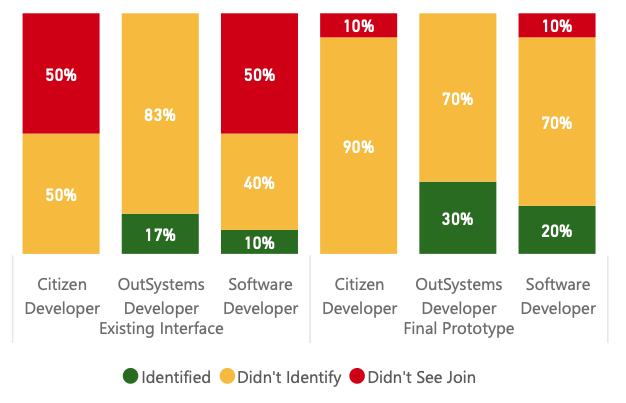
\includegraphics[width=0.5\linewidth]{left-join-with-null-readability-comparison}}%
    \subcaptionbox{Foreign key readability\label{fig:foreignKeyReadabilityComparison}}%
    {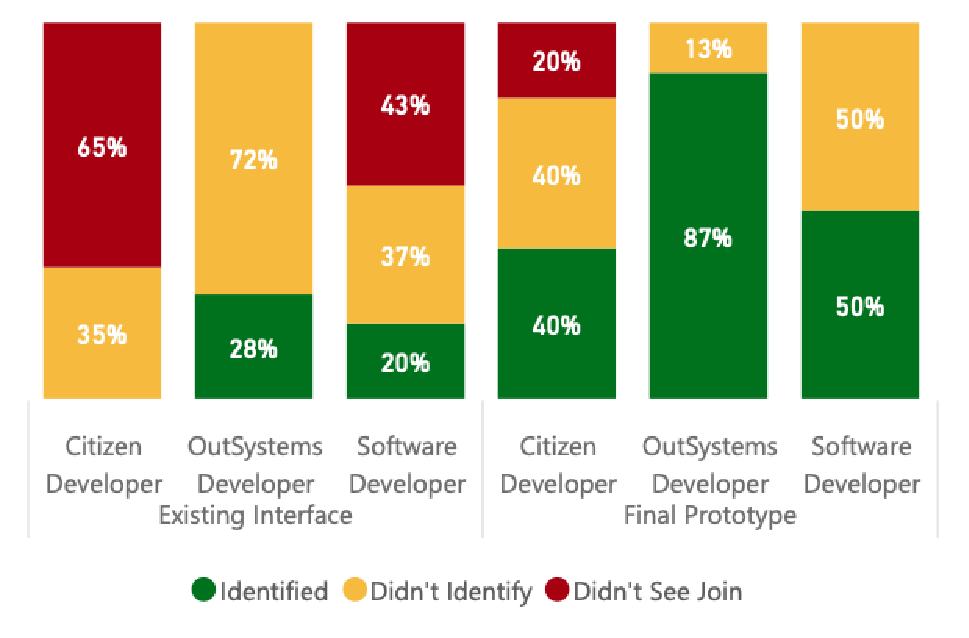
\includegraphics[width=0.5\linewidth]{foreign-key-readability-comparison}}%
    \caption{Comparison of the effectiveness between the Existing Interface and the Final Prototype, regarging specific use cases.}
    \label{fig:specificComparisons}
  \end{figure}

\begin{figure}[tb]
    \centering
    \subcaptionbox{Existing Interface\label{fig:susChartExistingInterface}}%
      {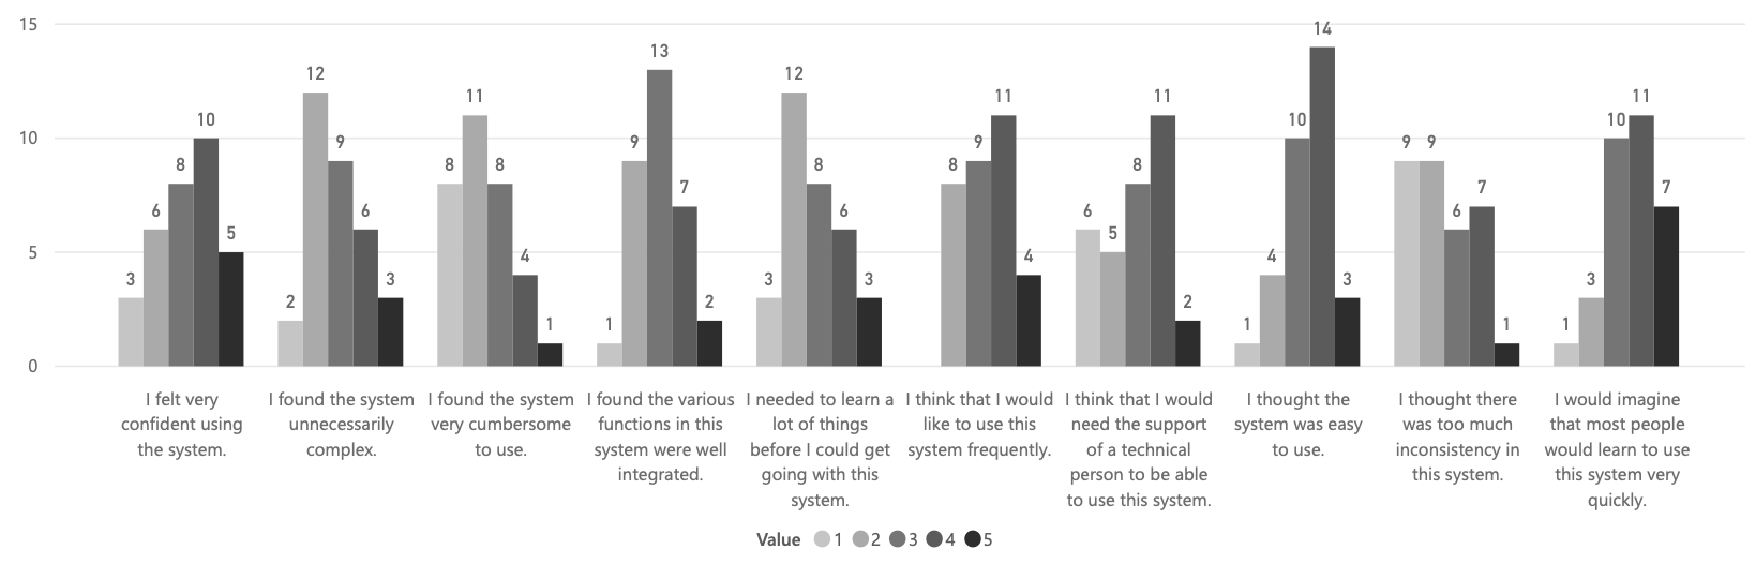
\includegraphics[width=1.0\linewidth]{sus-chart-existing-interface}}%
      \\
    \subcaptionbox{Final Prototype\label{fig:susChartFinalPrototype}}%
    {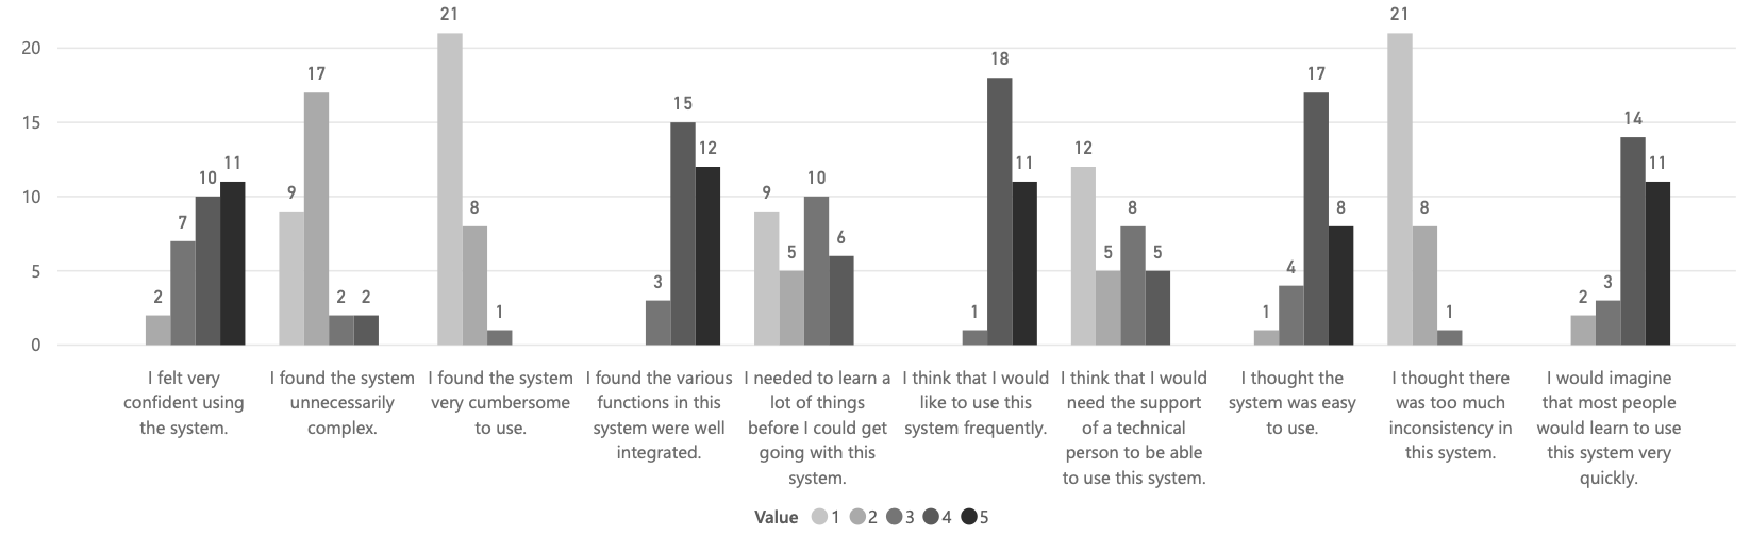
\includegraphics[width=1.0\linewidth]{sus-chart-final-prototype}}%
  \caption{Comparison of the System Usability Scale results (SUS) between the Existing Interface and the Final Prototype.}
    \label{fig:susChartComparison}
  \end{figure}

% Please add the following required packages to your document preamble:
% \usepackage{booktabs}
% \usepackage{multirow}
% \usepackage[table,xcdraw]{xcolor}
% If you use beamer only pass "xcolor=table" option, i.e. \documentclass[xcolor=table]{beamer}
\begin{table}[tb]
    \caption{Average and Standard Deviation of the System Usability Scale (SUS) results.}
	\label{tab:sus_results}
    \begin{tabular}{@{}|m{6cm}R{1.7cm}R{1.7cm}R{1.7cm}R{1.7cm}|@{}}
    \toprule
                                                                                               & \multicolumn{2}{l}{\textbf{Average}}                                                                                                           & \multicolumn{2}{l|}{\textbf{Standard Deviation}}                                                                                                \\ \cmidrule(l){2-5} 
    \multirow{-2}{*}{\textbf{Question}}                                                        & \multicolumn{1}{m{1.7cm}}{\cellcolor[HTML]{EFEFEF}\textbf{Existing Interface}} & \multicolumn{1}{m{1.7cm}}{\cellcolor[HTML]{E6E6E6}\textbf{Final Prototype}} & \multicolumn{1}{m{1.7cm}}{\cellcolor[HTML]{EFEFEF}\textbf{Existing Interface}} & \multicolumn{1}{m{1.7cm}|}{\cellcolor[HTML]{E6E6E6}\textbf{Final Prototype}} \\ \midrule
    I think that I would like to use this system frequently.                                   & \cellcolor[HTML]{EFEFEF}3.34                                            & \cellcolor[HTML]{E6E6E6}4.33                                         & \cellcolor[HTML]{EFEFEF}0.99                                            & \cellcolor[HTML]{E6E6E6}0.54                                          \\ \midrule
    I found the system unnecessarily complex.                                                  & \cellcolor[HTML]{EFEFEF}2.88                                            & \cellcolor[HTML]{E6E6E6}1.90                                         & \cellcolor[HTML]{EFEFEF}1.08                                            & \cellcolor[HTML]{E6E6E6}0.79                                          \\ \midrule
    I thought the system was easy to use.                                                      & \cellcolor[HTML]{EFEFEF}3.44                                            & \cellcolor[HTML]{E6E6E6}4.07                                         & \cellcolor[HTML]{EFEFEF}0.93                                            & \cellcolor[HTML]{E6E6E6}0.73                                          \\ \midrule
    I think that I would need the support of a technical person to be able to use this system. & \cellcolor[HTML]{EFEFEF}2.94                                            & \cellcolor[HTML]{E6E6E6}2.20                                         & \cellcolor[HTML]{EFEFEF}1.22                                            & \cellcolor[HTML]{E6E6E6}1.14                                          \\ \midrule
    I found the various functions in this system were well integrated.                         & \cellcolor[HTML]{EFEFEF}3.00                                            & \cellcolor[HTML]{E6E6E6}4.30                                         & \cellcolor[HTML]{EFEFEF}0.94                                            & \cellcolor[HTML]{E6E6E6}0.64                                          \\ \midrule
    I thought there was too much inconsistency in this system.                                 & \cellcolor[HTML]{EFEFEF}2.44                                            & \cellcolor[HTML]{E6E6E6}1.33                                         & \cellcolor[HTML]{EFEFEF}1.20                                            & \cellcolor[HTML]{E6E6E6}0.54                                          \\ \midrule
    I would imagine that most people would learn to use this system very quickly.              & \cellcolor[HTML]{EFEFEF}3.63                                            & \cellcolor[HTML]{E6E6E6}4.13                                         & \cellcolor[HTML]{EFEFEF}1.02                                            & \cellcolor[HTML]{E6E6E6}0.85                                          \\ \midrule
    I found the system very cumbersome to use.                                                 & \cellcolor[HTML]{EFEFEF}2.34                                            & \cellcolor[HTML]{E6E6E6}1.33                                         & \cellcolor[HTML]{EFEFEF}1.08                                            & \cellcolor[HTML]{E6E6E6}0.54                                          \\ \midrule
    I felt very confident using the system.                                                    & \cellcolor[HTML]{EFEFEF}3.25                                            & \cellcolor[HTML]{E6E6E6}4.00                                         & \cellcolor[HTML]{EFEFEF}1.20                                            & \cellcolor[HTML]{E6E6E6}0.93                                          \\ \midrule
    I needed to learn a lot of things before I could get going with this system.               & \cellcolor[HTML]{EFEFEF}2.81                                            & \cellcolor[HTML]{E6E6E6}2.43                                         & \cellcolor[HTML]{EFEFEF}1.13                                            & \cellcolor[HTML]{E6E6E6}1.12                                          \\ \bottomrule
    \end{tabular}
    \end{table}


\section{Future Work}
\label{sec:future_work}

\section{Conclusion} %final remarks
\label{sec:conclusion}
